\documentclass[a4paper]{article}

\usepackage{INTERSPEECH_v2}
\usepackage{multirow}

\title{Deep Neural Network Architectures for Double Talk Detection \\}
\name{Ziteng Wang$^1$, Co-author Name$^2$}
\address{
  $^1$Institute of Acoustics, University of Chinese Academy of Sciences, China\\
  $^2$INRIA Nancy, France}
\email{zwang@loria.fr, coauthor@company.com}

\begin{document}

\maketitle
%
\begin{abstract}
  In Acoustic Echo Cancellation (AEC), the adaptive filter diverges from its optimum solution when double talk occurs. In this paper, the problem of Double Talk Detection (DTD) is addressed from a machine learning perspective. The Deep Neural Network (DNN) is introduced as a binary classifier, which is trained on spectral features of the far-end speech and the microphone signal. To further make use of the available data, a separate network is proposed to learn the echo path effect. The network, which maps the far-end speech to its echo image, actually collaborates with the classifier. Experiments are conducted to show its performance and the robustness to environment changes is analyzed.
\end{abstract}
\noindent\textbf{Index Terms}: double talk detection, deep neural network, echo path, acoustic echo cancellation

\section{Introduction}

In a full-duplex system as illustrated in Fig.1, Acoustic Echo Cancellation (AEC) is an indispensable module which is used to suppress the undesirable echo of the far-end speech. An adaptive filter is designed to identify the echo path and then the echo component is subtracted from the microphone signal. If both the far-end speaker and the near-end speaker talk simultaneously, the so-called double talk occurs. The near-end speech acts as uncorrelated noise to the adaptive algorithm and diverges the filter from its optimum solution. Therefore Double Talk Detection (DTD) is introduced to control the updating of the adaptive filter. When double talk is detected, the filter update is slowed down or completely halted~\cite{benesty2011double}.

% heuristic
The solution to the DTD problem is a robust discriminator. The discriminator should achieve a high detection accuracy while keeping a low level of false alarm probability, regardless of the ambient noise and the changes in the echo path. In literatures, the common routine is to design a feature or detection statistic from the available signals. By comparing its value to a heuristic threshold, a binary decision is made: double talk or no double talk. The classical Geigel algorithm~\cite{duttweiler1978twelve} is based on an energy feature, which just involves the magnitudes of the recent past samples of the far-end speech. A generalized approach based on the Holder inequality is proposed in~\cite{paleologu2011class}, which takes the effect of noise into consideration. In~\cite{hamidia2014double}, a feature set is designed which includes the standard deviation and the log-energy of the signals. A large family of methods are based on the cross-correlation~\cite{ye1991new,schuldt2012delay,cho1999objective,benesty2000new,iqbal2007normalized} and the coherence~\cite{gansler1996double,tashev2012coherence}. The correlation statistic is usually calculated between the residual echo signal and the microphone signal~\cite{ye1991new}. However, it is shown vulnerable to the near-end disturbance and a time delay is introduced to improve the performance~\cite{schuldt2012delay}. Another option is the cross correlation between the far-end signal and the microphone signal~\cite{cho1999objective}. The Normalized Cross-Correlation (NCC) methods are discussed in~\cite{benesty2000new,iqbal2007normalized}. There are also other methods based on the signal envelop~\cite{szwoch2008low} and the zero-crossing rate~\cite{ikram2015double}, which are intended for the cases of low computational capacity.

The methods above generally exploit no prior information of the acoustic environment. While in many scenarios such as in a conference room, the positions of the loudspeaker and the microphone are fixed over time, the acoustic properties of the environment can then help the detection of a double talk instance. In~\cite{jung2005new}, the double talk decision is made with the estimated echo path. A known loudspeaker impulse response is assumed and utilized in~\cite{ahgren2005acoustic}. Besides, the fact that data samples can be easily obtained in these scenarios motivates data-driven methods. A learning based approach is proposed in~\cite{iqbal2006doubletalk}, which employs a one recurrent layer network. The GMM model is considered in~\cite{lee2010frequency} along with frequency domain features. Notably, the idea of deep learning already achieves success in many applications, such as in a similar task of Voice Activity Detection (VAD)~\cite{zhang2013deep,wang2015universal}, though VAD is designed to distinguish between speech and noise periods. One AEC related work is the residual echo suppression with Deep Neural Network (DNN) in~\cite{lee2015dnn}.

\begin{figure}[t]
  \centering
  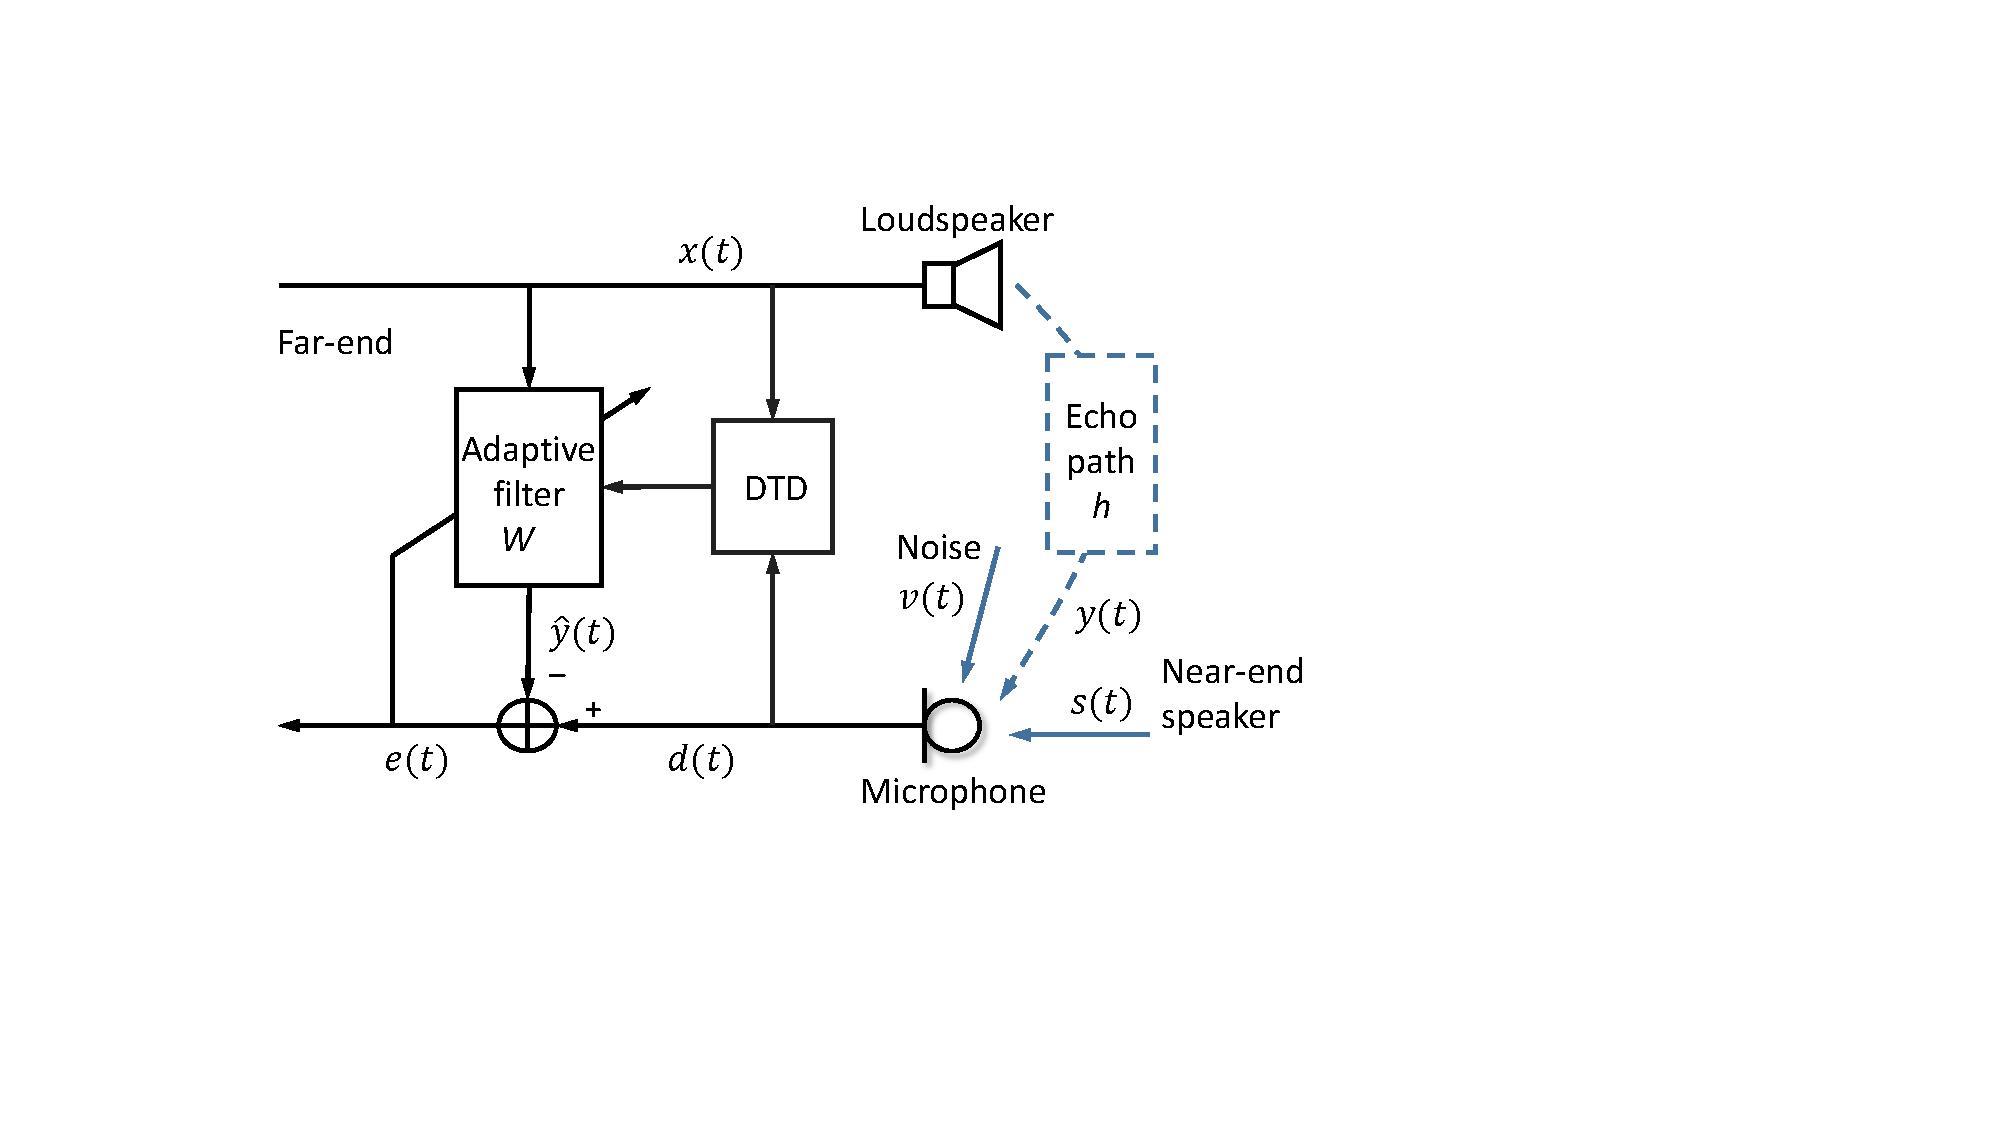
\includegraphics[width=0.95\linewidth]{fig1_aec.pdf}
  \caption{AEC in a full-duplex system. The DTD module controls the updating of the adaptive filter.}
  \label{fig1}
\end{figure}

In this paper, we apply the deep learning methodology to the DTD problem. The problem can be easily formulated as a binary classification task, for which DNN is introduced as a discriminative classifier. The available training samples can be further utilized by a separate network, which is proposed to learn the echo path effect. The far-end speech is mapped to its echo images. This network indeed collaborates with the classifier and benefits the performance. Especially, its functionality is different from the common practice of cancelling the echo effect as the network in~\cite{lee2015dnn}. And such a network is shown not proper for the task. Simulations are performed in the experiments and the behaviour of these networks is analyzed.

The outline of this paper is as follows. In section 2, the problem of DTD is defined. Section 3 introduces the proposed DNN based classifiers. The evaluation results are given in section 4 and conclusions are drawn in section 5.

\begin{figure*}[t]
  \centering
  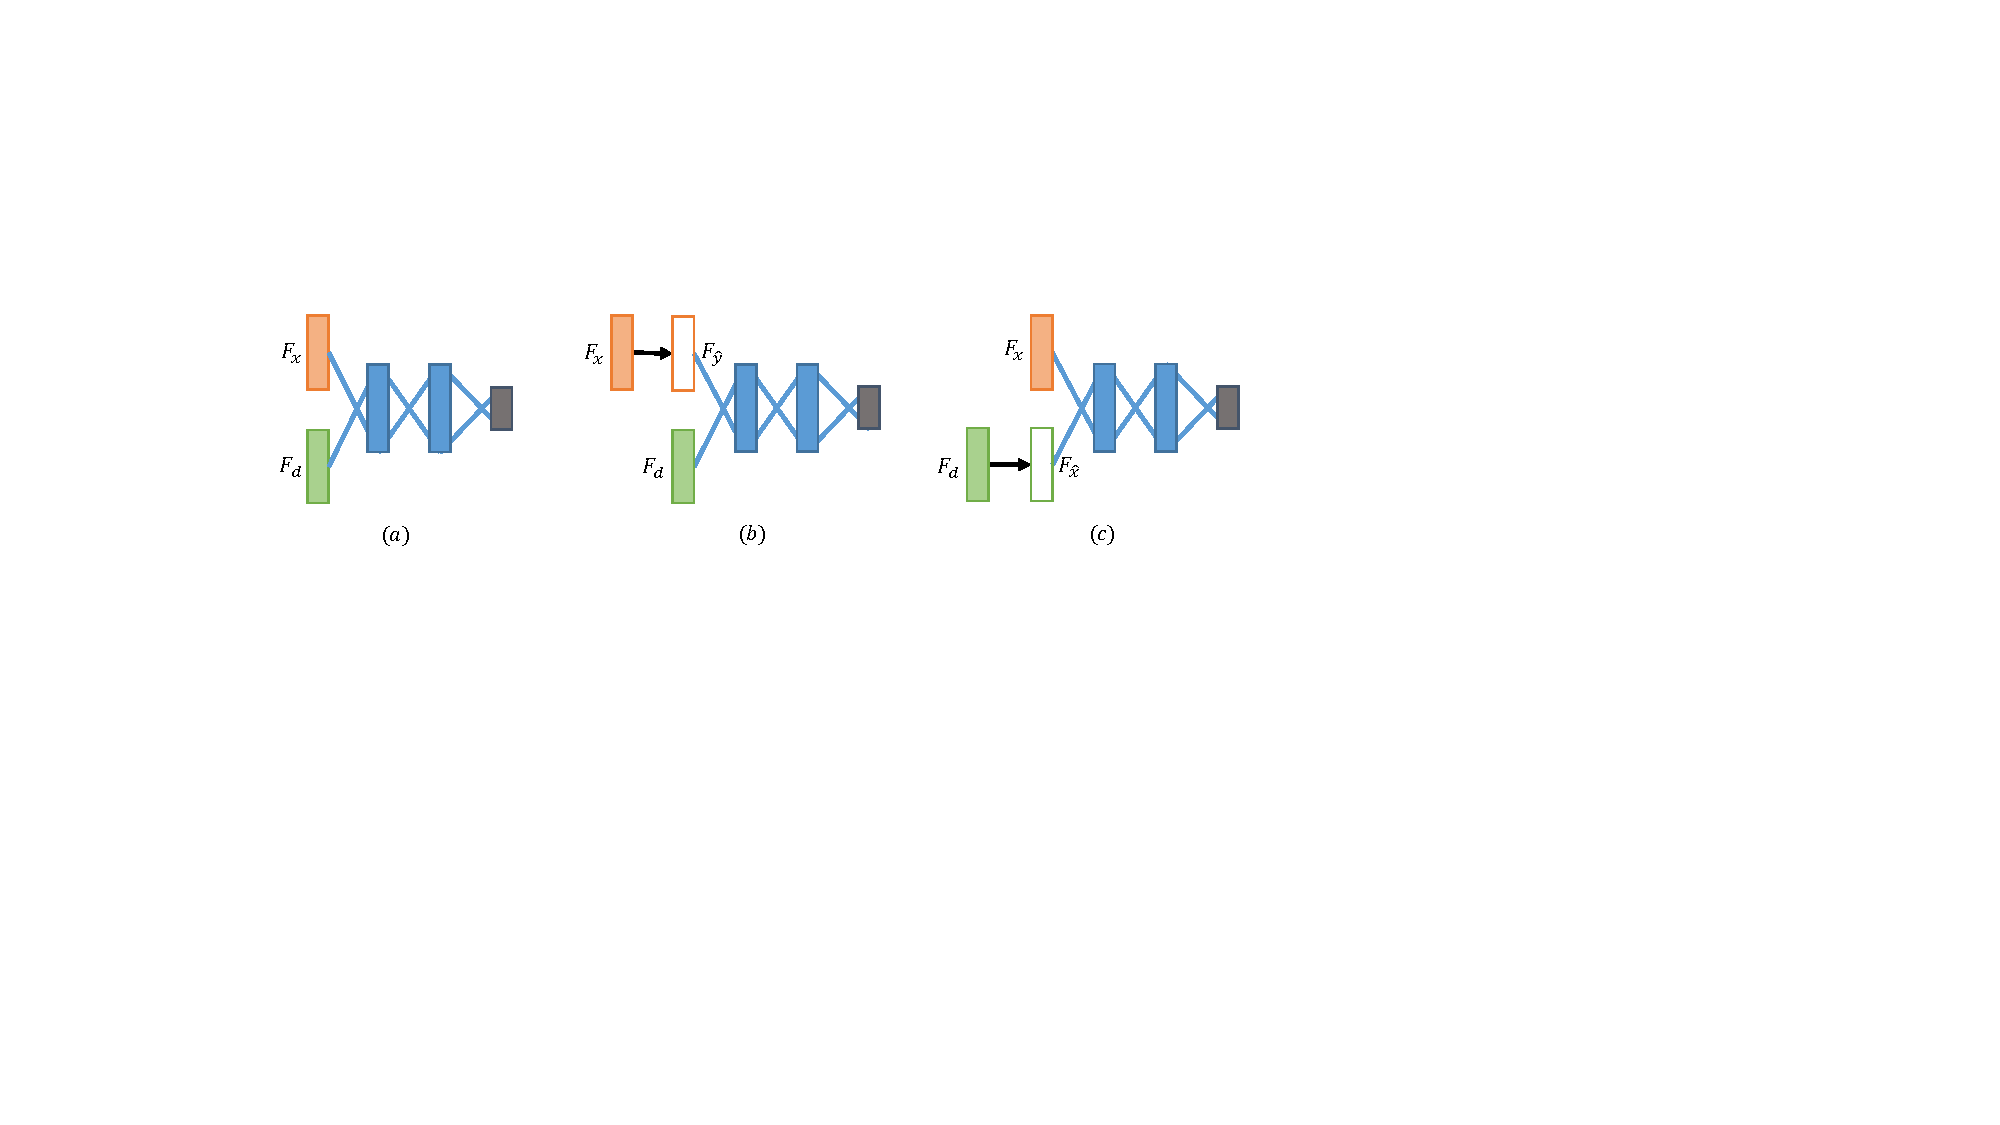
\includegraphics[width=0.9\linewidth]{fig2_nn.pdf}
  \caption{The proposed DNN architectures: (a) the binary classifier (b) the classifier with an echo learning net (c) the classifier with an echo suppression net.$F_x,F_d,F_y$ are respectively the feature vectors of the far-end signal, the microphone signal and the echo.}
  \label{fig2}
\end{figure*}

\section{Double talk detection}

As shown in Fig.1, the signal captured in the microphone is
\begin{equation}\label{eq:micsig}
  d(t)=y(t)+s(t)+v(t)
\end{equation}
where $t$ is the time index, $s(t)$ is the near-end speech, $v(t)$ is the ambient noise, and $y(t)$ is the echo of the far-end signal $x(t)$. $y(t)=h_L*h(t)*x(t)$ with $*$ denoting convolution and $h_L, h(t)$ being the loudspeaker response and the echo path response. The adaptive filter $\mat{W}$ is designed to identify the system response, so the echo can be estimated and then subtracted from the microphone signal. The residual signal is
\begin{equation}\label{eq:err}
  e(t) = d(t) - \mat{W}^T\mat{x}
\end{equation}
where $\mat{x}=[x(t)~x(t-1)~...~x(t-L+1)]^T$ and $^T$ denotes transpose.

When double talk occurs, $\mat{W}$ will diverge from its optimal value and tend to cancel the near-end speech. To detect double talk, two hypothesises are made
\begin{eqnarray}
% \nonumber % Remove numbering (before each equation)
  H_0:  s(t)=0, &\text{no double talk} \\
  H_1:  s(t)\neq 0,& \text{double talk}
\end{eqnarray}
Then a general inference procedure is

1) Design a detection statistic $\xi$ with the available signals, e.g. $x(t),d(t)$ and $e(t)$.

2) Compare $\xi$ to a preset threshold and make a binary decision: either $H_0$ or $H_1$.

3) Once $H_1$ is declared, the status is held for a minimum period and the filter update is disabled.

As an example, the NCC method in~\cite{iqbal2007normalized} is based on the following statistic
\begin{equation}\label{eq:ncc}
  \xi_{NCC}=1-\frac{r_{ed}}{\sigma^2_d}
\end{equation}
where $r_{ed}=\mathbb{E}[e(t)d(t)]$ and $\sigma^2_d$ is the variance of $d(t)$. $\mathbb{E}$ denotes expectation. The theoretical decision threshold is 1. If $\xi_{NCC}<1$, then double talk occurs.
%\begin{equation}\label{eq:ncc_benesty}
%  \xi_{NCC}=\sqrt{ \mat{r}^T_{\mat{x}d}(\sigma_d^2\mat{R}_{\mat{x}\mat{x}})^{-1}\mat{r}_{\mat{x}d} }
%\end{equation}
%where $\mat{R}_{\mat{x}\mat{x}}=\mathbb{E}\{\mat{x}\mat{x}^T\}$ is the autocorrelation matrix, $\mat{r}_{\mat{x}d}=\mathbb{E}\{\mat{x}d(t)\}$ is the cross correlation vector, $\sigma_d$ is the variance of $d(t)$ and $\mathbb{E}$ denotes expectation. The decision threshold is 1.


\section{The DNN architectures}

In the following, the DTD problem is considered as a binary classification task, which can be solved by learning from examples. DNN is employed to perform supervised training. The proposed network architectures are illustrated in Fig.2.

\subsection{Features and targets}

The input features are the logarithm of the filter-bank energy extracted from the far-end signal and the microphone signal. The calculation requires Short-time Fourier Transform (STFT), which in practice can be accomplished easily together with frequency domain AEC. And the frame shift is adjusted accordingly to give a timely response. The difference between the two signal features is also used. Suppose there are $K$ filter bands, then the input vector is of $3K$ in size, which is denoted as $\{\mat{F}_x, \mat{F}_d, \mat{F}_{x-d}\}$.

The output targets are defined by two vectors: $[1,0]^T$ for $H_0$ and $[0,1]^T$ for $H_1$. Two nodes are used rather than one so that discriminative training can be performed.

\subsection{Binary classifier}

DNN is mainly employed as a binary classifier as in Fig.2(a). It is a basic feed-forward network with all the layers linearly connected. The activation function is ReLU for the hidden layers and Softmax for the last layer. Cross-entropy is used as the loss function:
\begin{equation}\label{eq:ce}
  loss_{CE}=-\sum [p\text{log}(\hat{p})+(1-p)\text{log}(1-\hat{p})]
\end{equation}

\subsection{Echo learning}

The training data, specifically the date samples of class $H_0$, is further utilized in a separate echo learning network. A mapping from $\mat{F}_x$ to the echo image $\mat{F}_y$ is learned as in Fig.2(b) or an inverse mapping is learned as in Fig.2(c). A test sample is first processed by the mapping network and then sent to the classifier. We now investigate the features actually used for classifying the two classes. In the former case, the features are
\begin{displaymath}
H_0 : \left \{ \begin{matrix} \mat{F}_{\hat{y}} \\ \mat{F}_{y+v} \end{matrix} \right.
\quad H_1 : \left \{ \begin{matrix} \mat{F}_{\hat{y}} \\ \mat{F}_{y+s+v} \end{matrix} \right.
\end{displaymath}
where the difference feature vectors are omitted. Here the echo path effect and the nonlinearity introduced by the loudspeaker are partially handled by the echo learning network. An easier classification task is expected with a better learned mapping. In the latter case, the network learns to cancel the echo effect, which is a process commonly seen in echo suppression tasks. The features become
\begin{displaymath}
H_0 : \left \{ \begin{matrix} \mat{F}_{x} \\ \mat{F}_{\hat{x}+v'} \end{matrix} \right.
\quad H_1 : \left \{ \begin{matrix} \mat{F}_{x} \\ \mat{F}_{\hat{x}+s'+v'} \end{matrix} \right.
\end{displaymath}
Now a well trained echo suppression network should be robust to the noise and the near-end interferences, which may lead to a blurred decision surface between the two classes. The behavior of the two networks is shown in the experiments. During training, both mapping networks are tuned under the Mean Squared Error (MSE) criterion:
\begin{equation}\label{eq:mmse}
  loss_{MSE}=\sum |\hat{\mat{F}}-\mat{F}|^2
\end{equation}


\section{Experiment and analysis}

\subsection{Setup}

\begin{figure}[t]
  \centering
  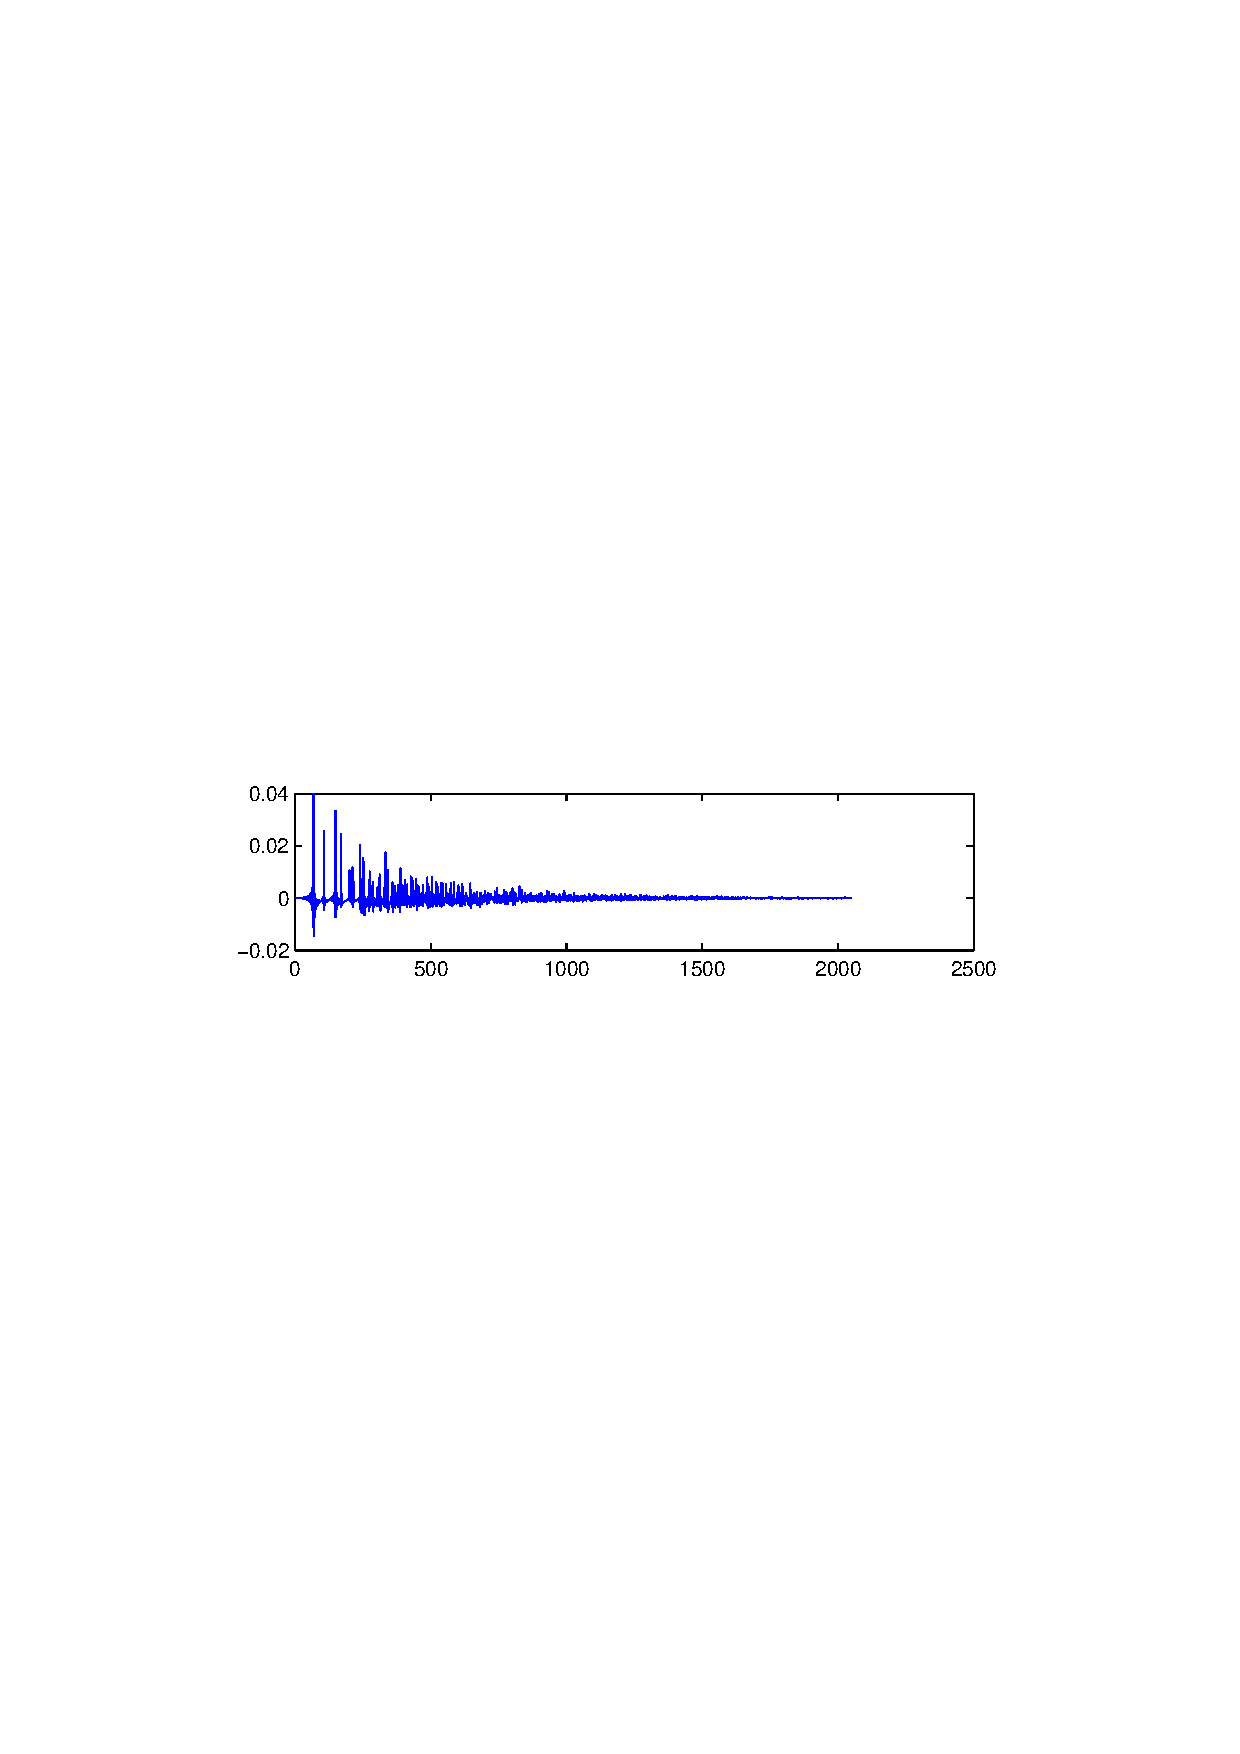
\includegraphics[width=\linewidth]{fig3_rir.pdf}
  \caption{The simulated echo path response.}
  \label{fig3}
\end{figure}

The experimental data comes from the TIMIT corpus. The speech sentences are sampled at 16 kHz. The echo path response is simulated in a room with reverberation time 230 ms. It is truncated to 2048 taps and shown in Fig.~\ref{fig3}. A moderate nonlinearity effect is considered in the loudspeaker, which is approximated with a memoryless sigmoidal function~\cite{comminiello2013functional}
\begin{equation}\label{eq:loud}
  z=\frac{2}{1+\exp(-a \cdot b)}-1
\end{equation}
where
\begin{equation}\label{eq:loudnl}
  b=1.5 \cdot x(t)-0.3 \cdot x^2(t)
\end{equation}
and the slop variable $a$ is set 2 for $x>0$ and 1 for $x<0$. 

The training and testing data is separately drawn from the train set and the test set. There are 2000 sentences for class $H_0$ and 800 sentences for $H_1$ since double talk instances are less frequent than no double talk instances. 160 sentences for each class are used as the development set. White Gaussian noise is added to the echo signal at Signal-to-Noise Ratio (SNR) of 30 dB. In the double talk case, the Near-end-to-Echo Ratio (NER) is set 0 dB. 100 sentences for each class are chosen for the final performance evaluation.

STFT is performed in 512 points with a 25 ms frame length and a 10 ms frame shift. 26 filter bands are used and only one frame is used as input. Then the binary classifier is 78-512-512-2 in size and the echo learning net is 26-512-512-26 in size. The mapping network is first trained and then fixed as a pre-processer for the classifier. In the training phase, the weight matrixes are initialized with i.i.d Gaussian samples and the bias vectors are filled with zeros. The Adam method is used for tuning the networks. Early stopping is applied when the loss in the development set no longer decreases. In the testing phase, the outputs of the classifier represent probabilities.

The metrics proposed in~\cite{cho1999objective} are used for evaluation: the probability of detection $P_d$ and the probability of false alarm $P_f$. In general, there exists a tradeoff between the two metrics and a higher $P_d$ is achieved at the cost of a higher $P_f$.

\subsection{Performance results}

The performance of the three networks proposed in section 3 are given by the Receiver Operating Characteristic (ROC) in Fig.\ref{fig4}. ROC is a curve of $P_d$ as the function of $P_f$. The Area Under the Curve (AUC) values are shown in the legends. A higher AUC indicates better performance. The three networks in Fig.2 are separately denoted as Anet, Bnet and Cnet. The NCC method~\cite{iqbal2007normalized} is included for comparison. An adaptation algorithm is needed in the NCC statistic calculation, for which the classical Normalized Least Mean Squares (NLMS)~\cite{haykin2002adaptive} is used. The filter $\mat{W}$ is updated as
\begin{equation}\label{eq:nlms}
  \mat{W}_{t+1}=\mat{W}_{t}+\mu \frac{e(t)\mat{x}}{\mat{x}^T\mat{x}+\delta}
\end{equation}
where $\mu=0.4$ and $\delta=0.001$ for numerical stability.

All the three networks outperform the NCC method and the Bnet performs best as expected. At a false alarm probability of 0.10, the basic classifier Anet achieves a 0.05 point higher accuracy than NCC. The Bnet is even 0.02 point better while the Cnet slightly deteriorates the performance of the classifier. The AUC scores of the networks are comparative, but still a difference is observed.

To support the arguments in subsection 3.3, the performance of the classifiers in each epoch is shown in   Fig.\ref{fig5}. The echo learning net is first trained. For each net with a decreased development error, it is saved and then a succeeding classifier is trained. For the Bnets, the detection accuracy goes up as the development error decreases. For the Cnets, though the development error decreases with more training epochs, the detection performance remains at a stable level.

\begin{figure}[t]
  \centering
  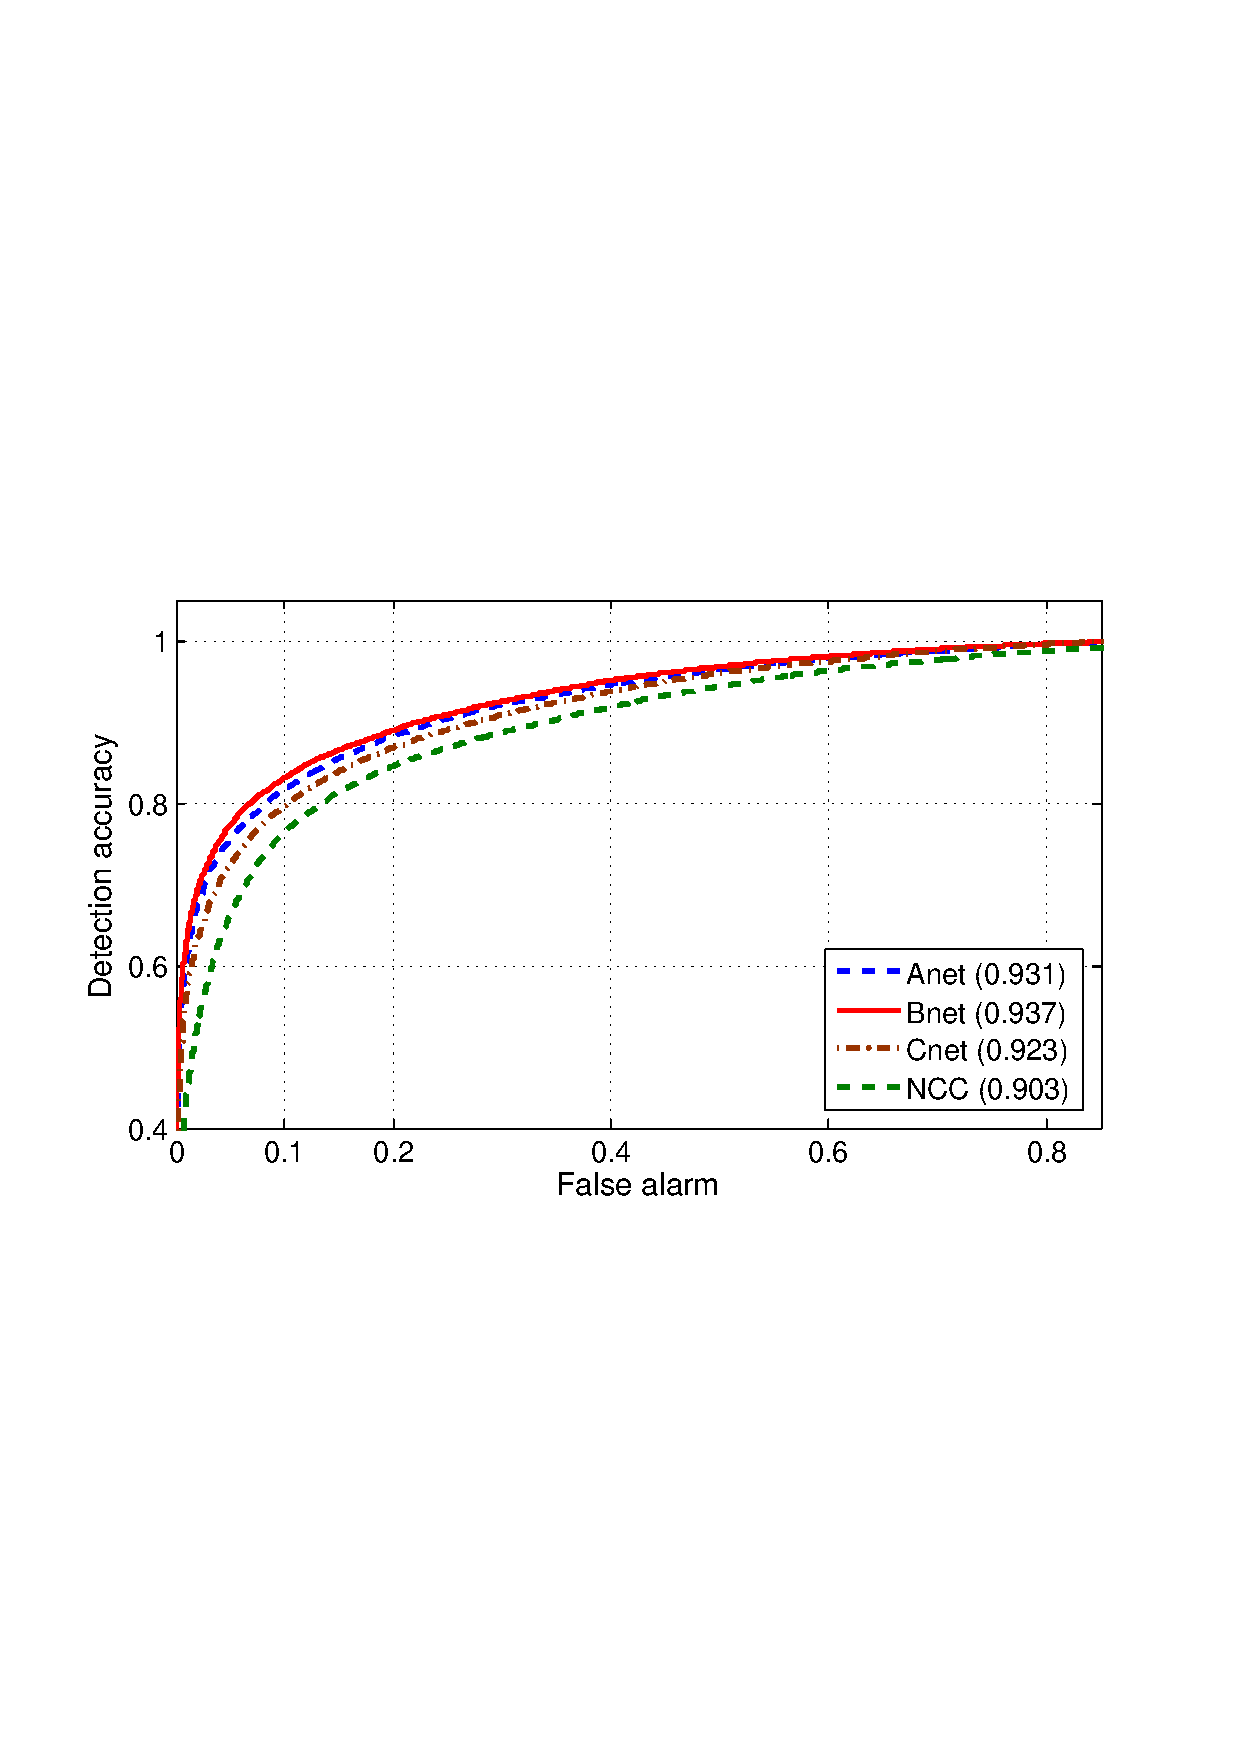
\includegraphics[width=0.95\linewidth]{fig4_roc.pdf}
  \caption{The ROC curve of the classifiers. The AUC values are shown in the legend.}
  \label{fig4}
\end{figure}
\begin{figure}[t]
  \centering
  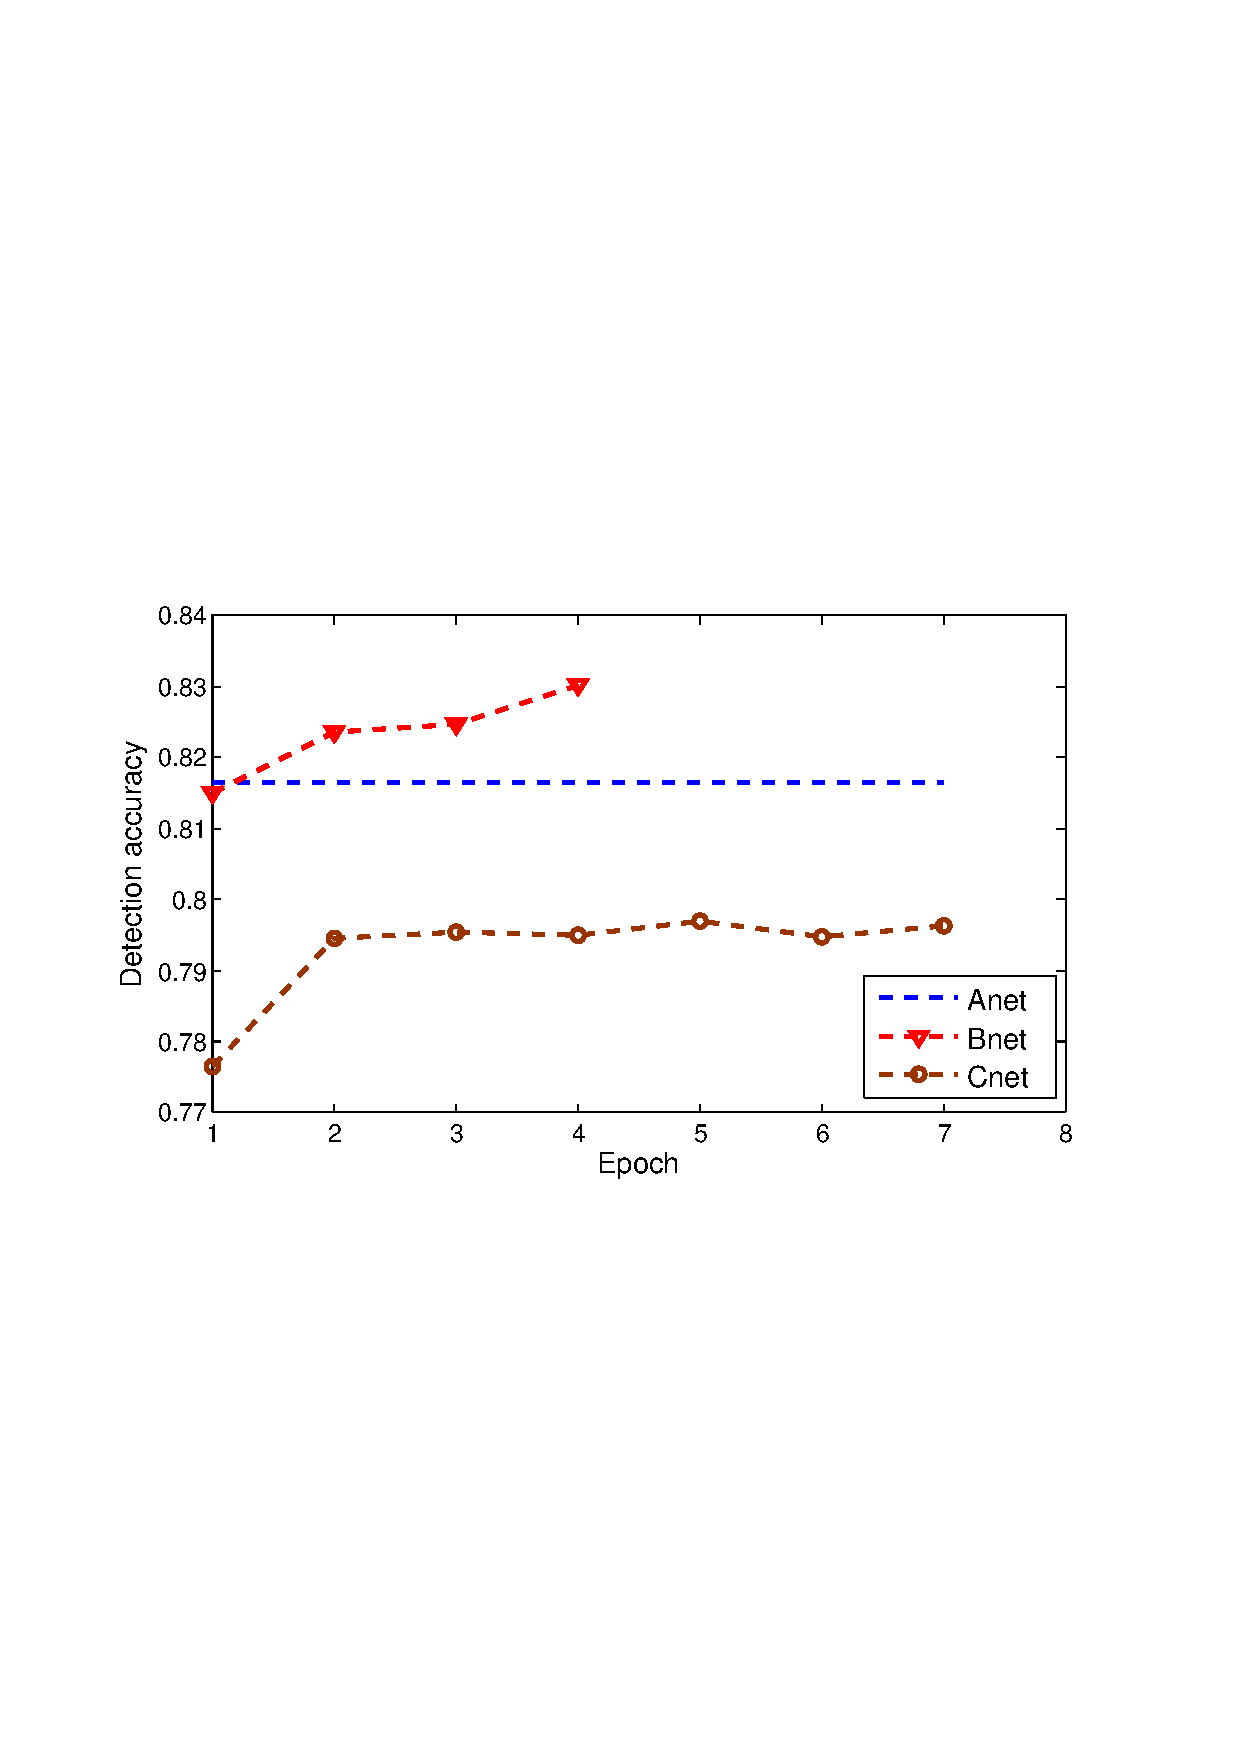
\includegraphics[width=0.95\linewidth]{fig5_epoch.pdf}
  \caption{The performance of the classifiers under $P_f=0.1$ as the development error decreases.}
  \label{fig5}
\end{figure}


\subsection{Environment robustness}

Note that the networks are trained in one single condition, they are tested for their generalization ability. The environment robustness test covers the near-end speech level, the ambient noise level and the variations in the echo path. The NER is changed from 0 dB to \{10, 5, -5\} dB, and the SNR is changed from 30 dB to \{35, 25, 20\} dB. The echo path variations are simulated by slightly changing both the position of the loudspeaker and the Reverberation Time (RT). The results of detection accuracy under a maximum false alarm rate 0.10 are given in Table~\ref{tab1}.

\begin{table}[th]
  \caption{The detection performance in changed environments under $P_f=0.1$.}
  \label{tab1}
  \centering
  \begin{tabular}{ r|c|c|c }
    \toprule
  \textbf{Case}~~~~~~ &  Anet & Bnet & Cnet   \\  \hline
  \text{baseline}~~~  & $81.7$  & $83.0$   & $79.6$      \\ \hline
   NER~~~$10$ dB   & $96.6$  & $96.8$   &  $95.3$      \\
        $5$ dB     & $91.9$  & $92.8$   &  $90.1$          \\
        $-5$ dB    & $71.6$  & $71.7$   &  $68.6$    \\  \hline
   SNR~~~$35$ dB   & $82.2$  & $82.6$   &  $79.4$  \\
        $25$ dB    & $79.2$  & $80.2$   & $77.6$   \\
        $20$ dB    & $72.8$  & $72.6$   & $71.6$        \\  \hline
   RT~~~$200$ ms   & $80.9$  & $79.7$   & $78.9$      \\
        $250$ ms   & $77.4$  & $76.3$   & $75.2$      \\
    \bottomrule
  \end{tabular}
\end{table}

Seen from the results, the trained networks favor easier tasks as indicated by high NER and high SNR. Overall, the Bnet stays ahead in performance. By increasing the near-end speech power just 5 dB higher than the echo, double talk is more accurately detected with about 10 percent improvements. However, the networks are also badly affected by low near-end speech power. Similar trends are observed in relative to SNR, though the fluctuations are smaller. In the RT test, it is found that the networks are tolerable to small changes in the echo path. When the changes become bigger, the mismatch in the echo learning network and the classifier begins to add, which lowers the accuracies.

%Finally, an test example is given in Fig.~\ref{fig6}.
%\begin{figure}[t!]
%  \centering
%  \includegraphics[width=0.95\linewidth]{fig6_example.pdf}
%  \caption{An test example.}
%  \label{fig6}
%\end{figure}

%\subsection{Performance in AEC}

%The double talk detectors are incorporated with the NLMS algorithm for echo suppression. The Echo Return Loss Enhancement (ERLE) loss is shown in the bottom.



\section{Conclusion}

In deep learning applications, a structured design is known beneficial to the final performance. In this paper, a separate echo learning net is combined with the DNN based classifier for the double talk detection problem. The echo learning net partially handles the nonlinearity in the system and collaborates with the classifier. The networks outperform conventional methods and they are shown robust to small changes in the environment. Future work includes multi-condition training and performance evaluation in AEC.

%\newpage

\section{Acknowledgements}

This work is supported by the China Scholarship Council (No. 201604910623). Experiments presented in this paper were carried out using the Grid'5000 testbed, supported by a scientific interest group hosted by Inria and including CNRS, RENATER and several Universities as well as other organizations (see $https://www.grid5000.fr$).


\bibliographystyle{IEEEtran}

\bibliography{mybib}

\end{document}
